\documentclass[11pt,psfig]{article}
\usepackage{epsfig}
\usepackage{times}
\usepackage{amssymb}
\usepackage{float}
\usepackage{listings}

\newcount\refno\refno=1
\def\ref{\the\refno \global\advance\refno by 1}
\def\ux{\underline{x}}
\def\uw{\underline{w}}
\def\bw{\underline{w}}
\def\ut{\underline{\theta}}
\def\umu{\underline{\mu}} 
\def\bmu{\underline{\mu}} 
\def\be{p_e^*}
\newcount\eqnumber\eqnumber=1
\def\eq{\the \eqnumber \global\advance\eqnumber by 1}
\def\eqs{\eq}
\def\eqn{\eqno(\eq)}

 \pagestyle{empty}
\def\baselinestretch{1.1}
\topmargin1in \headsep0.3in
\topmargin0in \oddsidemargin0in \textwidth6.5in \textheight8.5in
\begin{document}
\setlength{\parskip}{1.2ex plus0.3ex minus 0.3ex}


\thispagestyle{empty} \pagestyle{myheadings} \markright{Homework
1: CS 217 Spring 2015}



\title{CS 217 Homework 1}
\author{Zachary DeStefano, 15247592}
\date{Due Date: April 16, 2015}

\maketitle

\vfill\eject

\newpage

\section*{Problem 1}

Using our assumptions about lenses, we have the following diagram:

\begin{figure}[H]
\centering
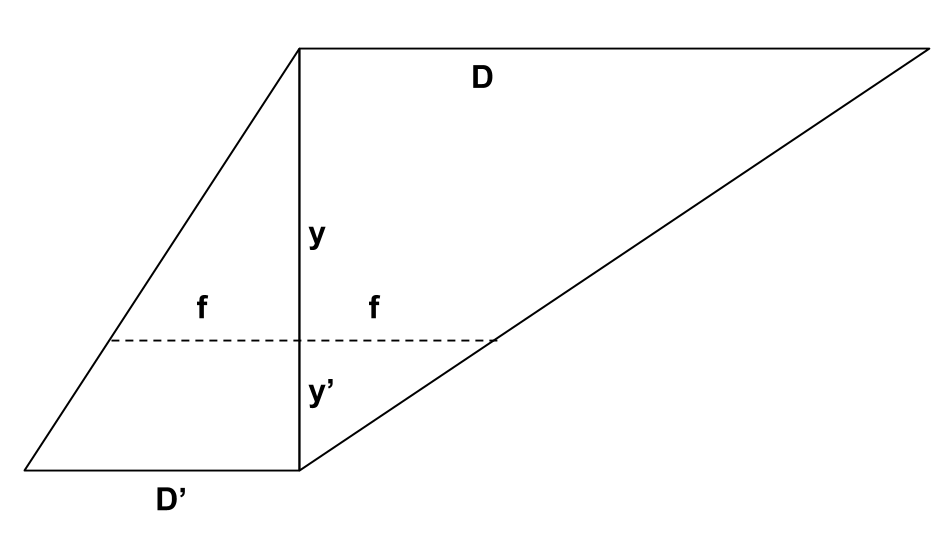
\includegraphics[height=4in]{hw1prob1diagram.png}
\caption{Diagram of lens and its focal length}
\end{figure}

The left side of the lens gives us the following equation using similar triangles
\[
\frac{y}{f} = \frac{y+y'}{D'}
\]
The right side of the length gives us the following equation using similar triangles
\[
\frac{y'}{f} = \frac{y+y'}{D}
\]
Adding together the two equations, we get the following
\[
\frac{1}{f} (y + y') = (\frac{1}{D} + \frac{1}{D'})(y + y')
\]
Cancelling the term $y+y'$ we end up with
\[
\frac{1}{f} = \frac{1}{D} + \frac{1}{D'}
\]
This is the thin lens equation


\section*{Problem 2}

Here is my triangulate.m function. It is also attached in the code folder. After running testtriangulation.m, the points matched almost exactly before noise was added and they were quite close after the noise was added.
\lstinputlisting[firstline=1, lastline=54]{triangulate.m}

\newpage

\subsection*{Part 1}

The following diagram illustrates the cross-section showing the horizontal and vertical field of view along with the focal length. The field of view will be $2\theta$

\begin{figure}[H]
\centering
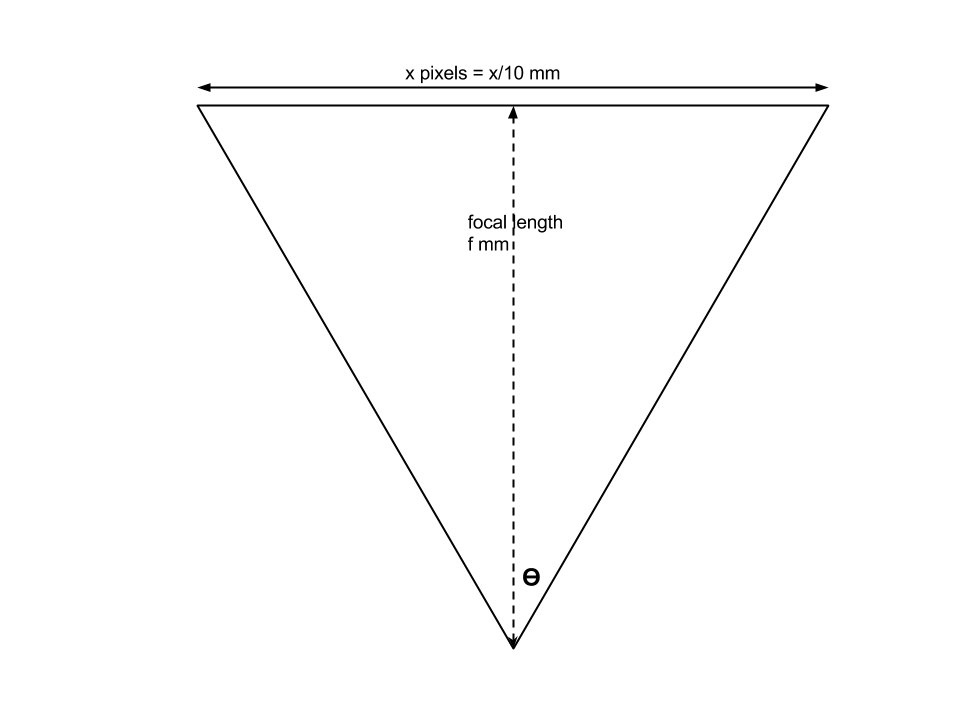
\includegraphics[height=4in]{hw1prob2drawing1.png}
\caption{Diagram of focal length and horizontal/vertical field of view}
\end{figure}
\newpage
Using trigonometry, it is easily observed that
\[
\theta = arctan(\frac{x}{20f})
\]
For the horizontal field of view, $x=640$\\
For the vertical field of view, $x=480$ \\
\\
When $f=50$, the horizontal field of view (in degrees) is as follows: 
\[
2arctan(\frac{640}{20 \cdot 50}) = 65.2385
\]
The vertical field of view (in degrees) is as follows:
\[
2arctan(\frac{480}{20 \cdot 50}) = 51.2820
\]
\\
When $f=100$, the horizontal field of view (in degrees) is as follows: 
\[
2arctan(\frac{640}{20 \cdot 100}) = 35.4893
\]
The vertical field of view (in degrees) is as follows:
\[
2arctan(\frac{480}{20 \cdot 100}) = 26.9915
\]

\newpage

\subsection*{Part 2}

A rotation of $\theta$ about the y axis has the following form
\[ \left( \begin{array}{ccc}
cos(\theta) & 0 & sin(\theta) \\
0 & 1 & 0 \\
-sin(\theta) & 0 & cos(\theta) \end{array} \right)\]
For us, $\theta=-45$ degrees, and we need homogeneous coordinates, thus our matrix $R$ is the following
\[ \left( \begin{array}{cccc}
1/\sqrt{2} & 0 & -1/\sqrt{2} & 0 \\
0 & 1 & 0 & 0\\
1/\sqrt{2} & 0 & 1/\sqrt{2} & 0 \\
0 & 0 & 0 & 1 \end{array} \right)\]
Translating to the right by 1 is the same as moving by one unit along the positive x-axis, which has the following matrix T 
\[ \left( \begin{array}{cccc}
1 & 0 & 0 & 1 \\
0 & 1 & 0 & 0\\
0 & 0 & 1 & 0 \\
0 & 0 & 0 & 1 \end{array} \right)\]
Since we are translating to the right after rotation, we have to apply the matrix $T$ in the new rotated coordinated system, thus to go from original world coordinate to final ones, you need to compute $RT$ which ends up being
\[ \left( \begin{array}{cccc}
1/\sqrt{2} & 0 & -1/\sqrt{2} & 1/\sqrt{2} \\
0 & 1 & 0 & 0\\
1/\sqrt{2} & 0 & 1/\sqrt{2} & 1/\sqrt{2} \\
0 & 0 & 0 & 1 \end{array} \right)\]
For $(1,1,1)$ in the world coordinate system, let $p$ be the homogenous version of the point, so 
\[
p=(1,1,1,1)^T
\]
In order to find its coordinates in the new system, we need to find a vector $x$ such that $RTx=p$ thus 
\[
x=(RT)^{-1} p
\] 
After computing $x$ it turns out the point in the new coordinate system is as follows
\[
(\sqrt{2} - 1, 1,0)
\]

\newpage

\subsection*{Part 3}

For this problem, I will assume that $y=z=0$ for my left and right eye in the world coordinate system. I will assume that both eyes are 2 cm away from the bridge of my nose. Thus the left eye has $x=-2$ and the right eye has $x=2$. Since I am looking at a computer monitor 40 cm away, I will also assume that I am looking at the point $(0,0,40)$ in the world coordinate system when estimating parameters. Here is a view from the top of my design:
\begin{figure}[H]
\centering
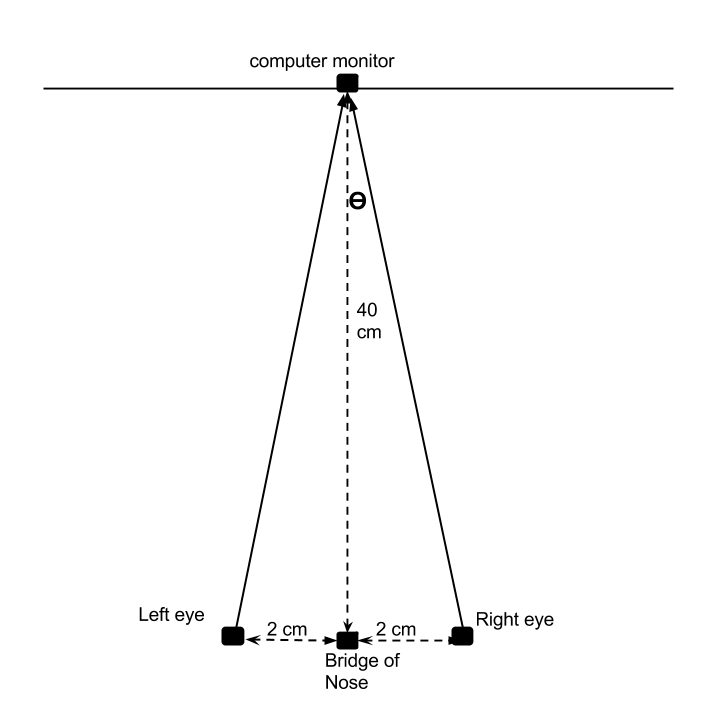
\includegraphics[height=4in]{hw1prob2drawing2.png}
\caption{Diagram eye and monitor locations}
\end{figure}
We can easily specify the two translation vectors $t_{left}$ and $t_{right}$\\
\[
t_{left} = (2,0,0)^T
\]
\[
t_{right} = (-2,0,0)^T
\]
\\
We now just need the two rotation matrices $R_{left}$ and $R_{right}$ to finish estimating extrinsic parameters. 
\newpage
The right eye will rotate counter-clockwise by $\theta$ to look at the center point. The left will rotate clockwise by the same amount, so it will rotate by $-\theta$.\\
\\
$R_{right}$ will be the following:
\[ \left( \begin{array}{ccc}
cos(\theta) & sin(\theta) & 0  \\
-sin(\theta) & cos(\theta) & 0 \\
0 & 0 & 1
 \end{array} \right)\]
$R_{left}$ will be the following:
\[ \left( \begin{array}{ccc}
cos(\theta) & -sin(\theta) & 0  \\
sin(\theta) & cos(\theta) & 0 \\
0 & 0 & 1
 \end{array} \right)\]
From the diagram you can tell that 
\[
sin(\theta) = \frac{1}{\sqrt{401}} \approx 0.04993
\]
\[
cos(\theta)=\frac{20}{\sqrt{401}} \approx 0.99875
\]
\newpage
\subsection*{Part 4}

As it turns out, noise in the pixel locations greatly increases the error in the recovered values. As the noise increases, the error increases in almost a linear fashion. Here is the code I used to test this. The arrays X,xL, and xR are the data points from the triangulation test script of the hemisphere. This code is also in the code folder as prob2part4.m.
\lstinputlisting[firstline=49, lastline=64]{prob2part4.m}
This is the resulting plot:
\begin{figure}[H]
\centering
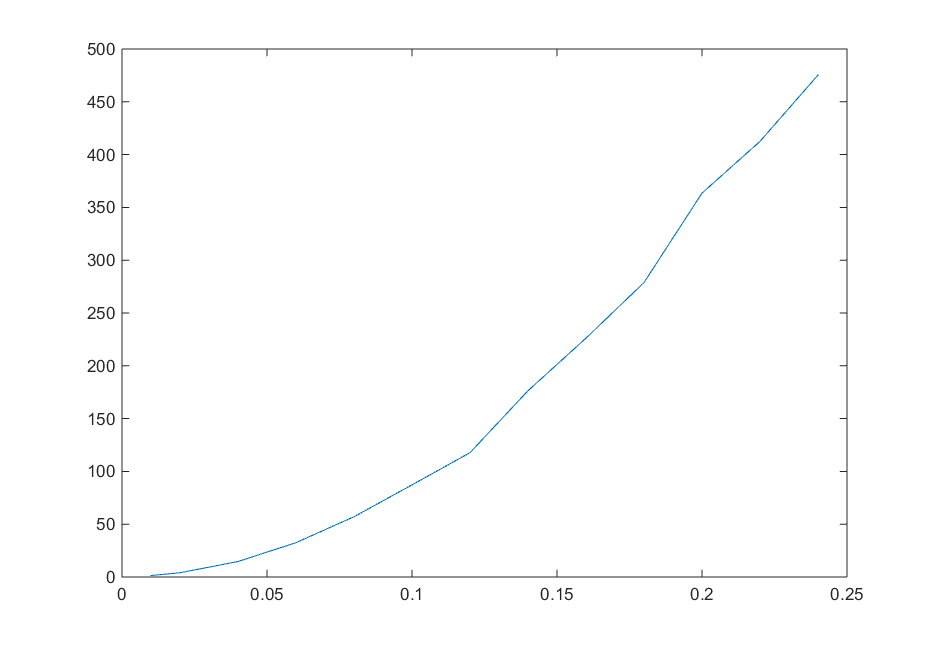
\includegraphics[height=3in]{prob2part4plot.png}
\caption{Sum of Squared Errors as function of amount of noise inserted}
\end{figure}

\newpage

\subsection*{Part 5}

In order to see how sensitive each of these were, I ran 50 tests for each part A to D and each test had a random variation of that specific camera parameter. I looked at the error for each test and averaged the errors together. These were my results:\\
\\
\begin{tabular}{ r |l }
Parameter changed & Average Sum of Squared Errors\\
  \hline                       
  Camera Center & 403.8366  \\
  Focal Length & 19.56 \\
  Camera Location & 4.1943e4 \\
  Rotation Angle & 2.34e6
\end{tabular}
\\
\\
As it turns out, the greatest amount of error comes from varying the rotation angle. \\
\\
Instead of specifying specific units and the amounts for those units, we should be specifying the percent error possible in the camera parameters. \\
\\
For Camera Center, we would specify a percentage of the image plane that the center could vary by\\
For Focal Length, we would specify a percentage of the focal length that the camera could vary by\\
For Camera Location, we would look at the range of $x,y,z$ values in the real woord coordinate system. You would then specify a percentage and the amount in each dimension that the camera location is allowed to vary by would be a percentage of the range found.\\
\\
For Rotation Angle, we could still specify a number of degrees since that is a fixed percentage of the allowed range of angles.\\
\\
Here is the code I used to generate the numbers above. The beginning of it generated x, xL, and xR. The code is also in the code folder as prob2part5.m.
\lstinputlisting[firstline=49, lastline=142]{prob2part5.m}

\newpage


\section*{Problem 3}

Here is my calibrate.m function. It is also in the code folder. 
\lstinputlisting[firstline=1, lastline=55]{calibrate.m}
It uses the function rq.m that I found on the internet and was written by a professor at NYU. That function is also in the code folder.
\lstinputlisting[firstline=1, lastline=27]{rq.m}

\subsection*{Part 1}

I used the following code to generate the data set and then test the calibrate function:
\lstinputlisting[firstline=1, lastline=85]{test_calibration.m}
All of the differences ended up being trivial and were likely due to floating point error, thus the function itself works very well. \\
\\
I then introduced noise as was done in the function. I used the noisy pixel locations and kept the original 3D locations to see what camera parameters were obtained. The original script used a noise factor of 0.01. I decided to also use 0.02 and 0.1 as noise factors to see what increasing noise does to the parameters. Here was my script:
\lstinputlisting[firstline=89, lastline=120]{test_calibration.m}

I then compared the parameters obtained using the output. In order from original $K$ matrix to the recovered K matrix as it gets noisier, here are the $K$ matrices:
\begin{verbatim}
   100     0    50
     0   100    50
     0     0     1

  100.0364    0.0014   49.9896
         0  100.0330   49.9683
         0         0    1.0000

  100.0540   -0.0030   49.9785
         0  100.0624   50.0167
         0         0    1.0000

   99.8103    0.0289   50.1466
         0   99.8229   50.5030
         0         0    1.0000
\end{verbatim}

As can be observed, the pixel magnification factors do start to vary as noise is increased but not by much. The pixel center location also starts to vary, but not by much. The skew factor however becomes non-zero suggesting that it appears there is skew in the lens when there is noise. 
\newpage
Doing the same thing but for the $R$ matrices, here are the rotation matrices obtained

\begin{verbatim}
    0.9998         0    0.0200
         0    1.0000         0
   -0.0200         0    0.9998

    0.9998    0.0000    0.0199
   -0.0000    1.0000   -0.0003
   -0.0199    0.0003    0.9998

    0.9998   -0.0000    0.0199
    0.0000    1.0000    0.0000
   -0.0199   -0.0000    0.9998

    0.9998    0.0002    0.0207
   -0.0002    1.0000    0.0033
   -0.0207   -0.0033    0.9998
\end{verbatim}
As can be observed, the rotation matrix does start to vary from the original but not by too much as the pixel locations get noisier. \\
\\
Lastly, I compared the camera location parameter t. Since it was a vector, I lined by the vectors obtained in order from left to right by amount of noise in test. This was the result:

\begin{verbatim}
   -0.2000   -0.1991   -0.1999   -0.1965
         0    0.0002    0.0014    0.0017
         0   -0.0008    0.0019   -0.0305
\end{verbatim} 

The camera location parameter obtained does start to increasingly vary as noise increases. Again though, the small amount of noise we introduced did not change it a whole lot. \\
\\
All of the code for this part is included in the file prob3part1.m in the code folder. 

\newpage

\subsection*{Part 2}

This is the code I used to test it on image 1:
\lstinputlisting[firstline=1, lastline=21]{prob3part2.m}
I ended up getting the following error:
\begin{verbatim}
Warning: Matrix is singular, close to singular or badly scaled.
         Results may be inaccurate. RCOND = NaN. 
\end{verbatim}
As it turns out, performing the SVD on our matrix fails to find the proper vector $c$ that indicates a calibration matrix. The last column of the $V$ matrix is all 0 values except for a -1 in the second to last entry. This likely occured because every point in the 3D coordinates has the same $z$ value so there are many possible placements of the camera and the image plane. The 0 values result from the fact that the equation is not linearly independent. \\
\\
The linear dependence comes from the fact that we have a plane in 3D. Thus we can place the image plane wherever we want and then find the other camera parameters. Likewise, we can place the camera wherever we want and then come up with a proper image plane. 

\subsection*{Part 3}

After running the program on the first image, it was able to extract these grid points:
\begin{figure}[H]
\centering
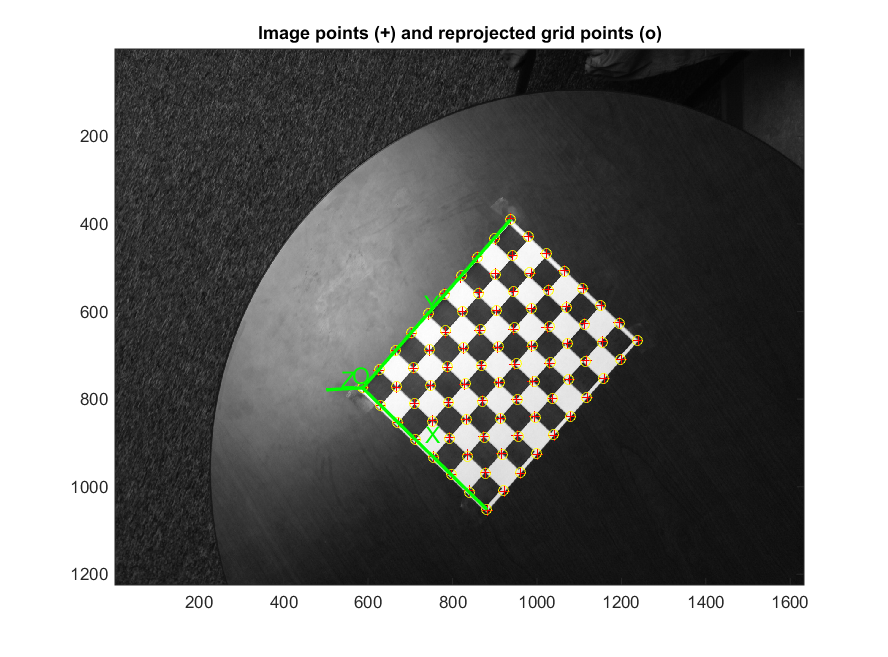
\includegraphics[height=4in]{prob3plot1.png}
\caption{Results for Image 1}
\end{figure}
\begin{figure}[H]
\centering
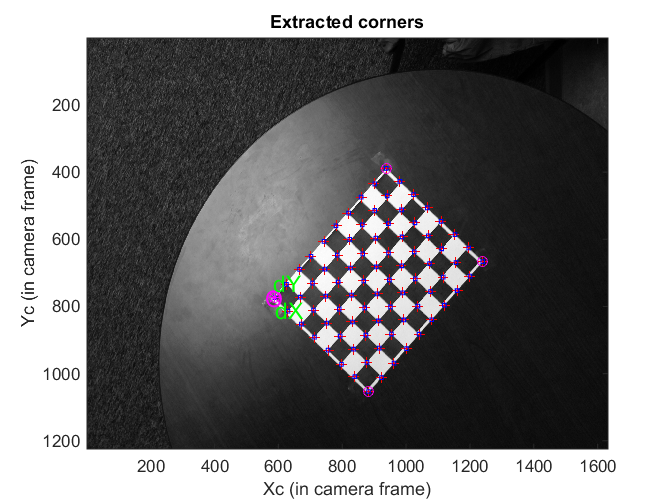
\includegraphics[height=4in]{prob3plot2.png}
\caption{Results for Image 1}
\end{figure}
I continued specifying corners for the rest of the images and these were the instrinsic parameters that resulted:
\begin{verbatim}
Calibration results (with uncertainties):

Focal Length:          fc = [ 1602.72820   1627.13289 ] ± [ 75.45401   76.76484 ]
Principal point:       cc = [ 830.78219   563.59275 ] ± [ 41.54681   54.40452 ]
Skew:             alpha_c = [ 0.00000 ] ± [ 0.00000  ]   
									=> angle of pixel axes = 90.00000 ± 0.00000 degrees
Distortion:            kc = [ 0.61729   -2.11774   -0.01065   0.02242  0.00000 ] 
									± [ 0.20311   1.40105   0.01976   0.01779  0.00000 ]
Pixel error:          err = [ 3.59673   2.89028 ]

Note: The numerical errors are approximately three times the standard deviations (for reference).

\end{verbatim}
Here is the extrinsic matrix visual
\begin{figure}[H]
\centering
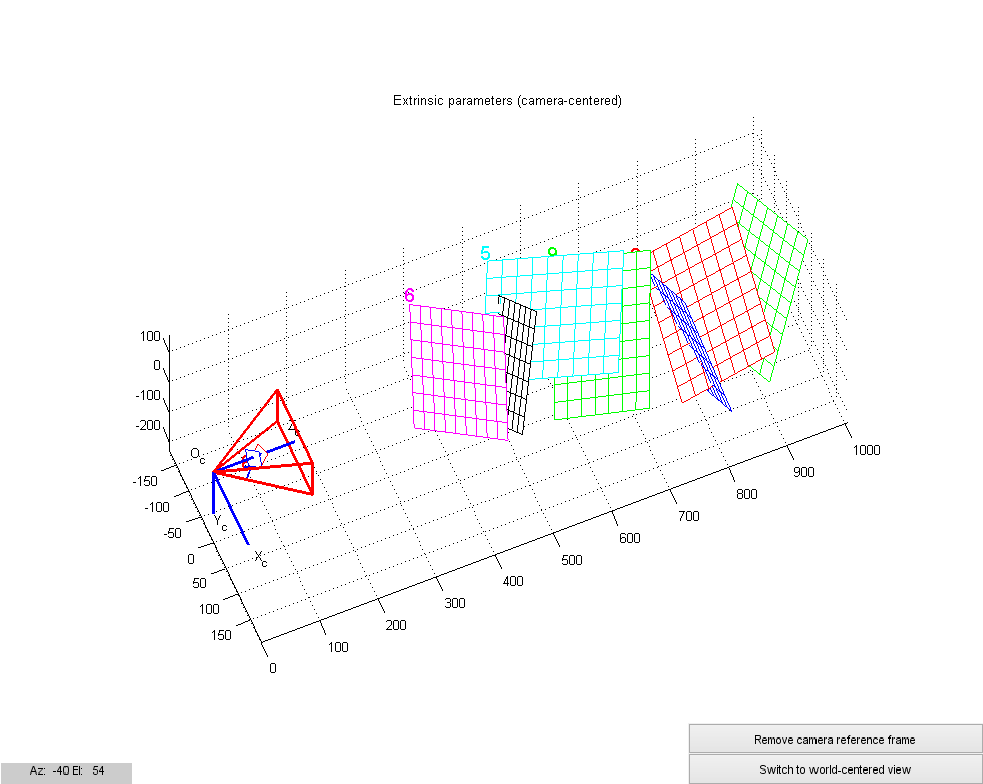
\includegraphics[height=4in]{prob3plot3.png}
\caption{Extrinsic parameters with single camera}
\end{figure}
\begin{figure}[H]
\centering
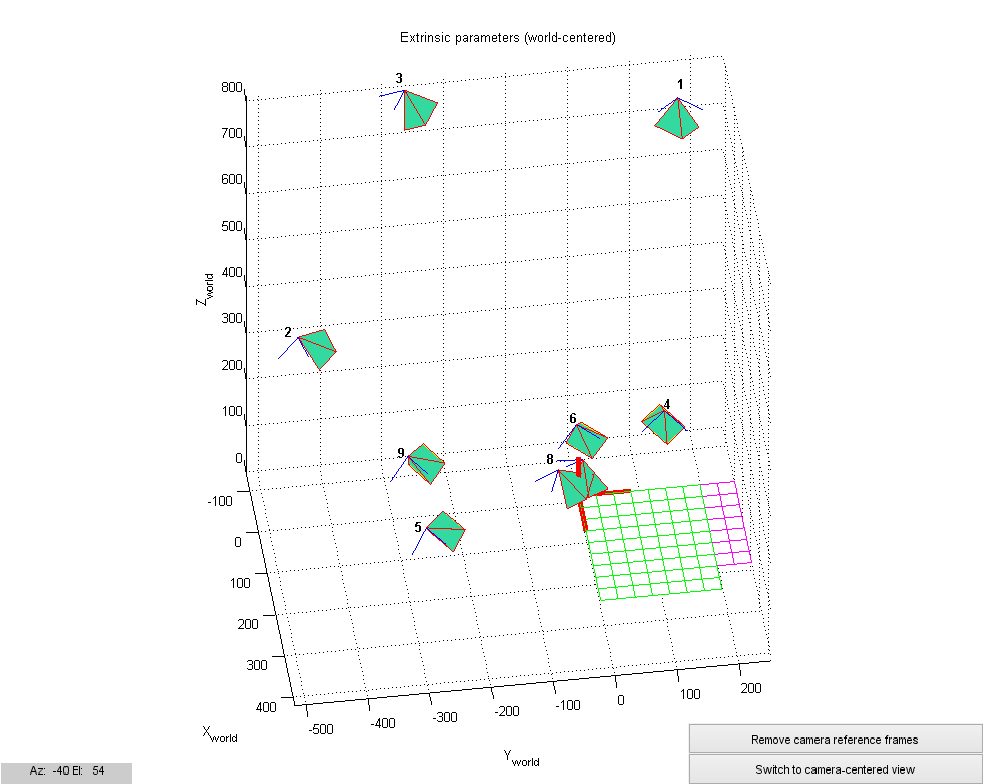
\includegraphics[height=4in]{prob3plot4.png}
\caption{Extrinsic parameters with world viewpoint}
\end{figure}

When running this program, it ran through all the images and thus had many more points to use. Some of the differences that occured were likely the result of how the data was brought into the program. In some of the images, the grid corners were not very accurate whereas in other ones they were quite accurate. Also, the program labelled X and Y somewhat arbitrarily.

\newpage

\subsection*{Part 4}

Here are my estimated dimensions:\\
length = 15.0212\\
width = 3.4682\\
height = 0.6473\\

\begin{figure}[H]
\centering
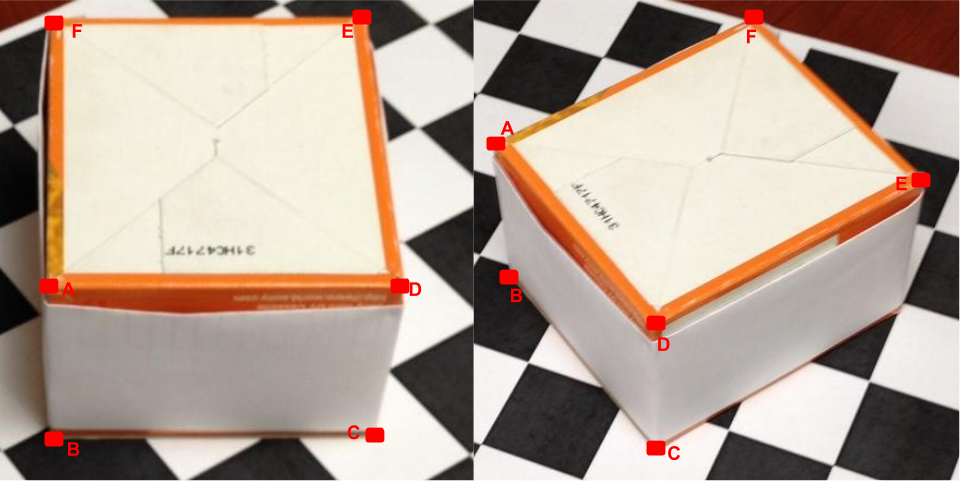
\includegraphics[height=4in]{hw1prob3diagram.png}
\caption{The points used to acquire dimensions}
\end{figure}

Here is the matlab code used to get the dimensions
\lstinputlisting[firstline=1, lastline=97]{prob3part4.m}

\end{document}








